%
%  Vincent Yannello
%
\documentclass[12pt,fullpage]{article}
\usepackage{fullpage}
\usepackage{psfrag}                                          % LaTeX graphics tool
\usepackage{pslatex}                                         % avoids the default cmr font
\usepackage{graphicx}                                        % graphics package 
\usepackage{epsfig}                                          % figures
\usepackage{hyperref}
\usepackage{color}

\begin{document}

\noindent
{\bf Power distribution} (from \color{blue}\url{http://www.math.wm.edu/~leemis/chart/UDR/UDR.html}\color{black})

\noindent
The shorthand $X \sim {\rm power}(\alpha,\, \beta)$ is used to indicate that the
random variable $X$ has the power distribution with parameters $\alpha$ and $\beta$.
A power random variable $X$ with positive scale parameter $\alpha$ and positive shape parameter $\beta$ has probability density function 
$$
f(x) = \frac{\beta x ^ {\kern 0.08 em \beta - 1}} {\alpha ^ {\kern 0.08 em \beta}} \qquad \qquad 0 < x < \alpha.
$$
The probability density function with $\alpha = 1$ and two different values of $\beta$ is illustrated below.
{\begin{figure}[h!]
\begin{center}
\psfrag{lab1}{$\beta = 0.5$}
\psfrag{lab2}{$\beta = 3$}
\psfrag{labx}{$x$}
\psfrag{labf}{$f(x)$}
\includegraphics[width=3.2in]{PowerPlot.ps}
\end{center}
\end{figure}}\\
The cumulative distribution function on
the support of $X$ is
$$
F(x) = P(X \le x) = \frac{x ^ {\kern 0.08 em \beta}} {\alpha ^ {\kern 0.08 em \beta}}  \qquad \qquad 0 < x < \alpha.
$$
The survivor function on the support of $X$ is
$$
S(x) = P(X \ge x) = 1 - \frac{x ^ {\kern 0.08 em \beta}} {\alpha ^ {\kern 0.08 em \beta}}  \qquad \qquad 0 < x < \alpha.
$$
The hazard function on the support of $X$ is
$$
h(x) = \frac{f(x)} {S(x)} = \frac {{\beta} \, {x} ^ {{\kern 0.08 em \beta} - 1}{{ \alpha}} ^ {-{\kern 0.08 em \beta}}} {\alpha^{\beta} - x^{\beta}} \qquad \qquad 0 < x < \alpha.
$$
The cumulative hazard function on the support of $X$ is
$$
H(x) = - \ln S(x) = -\ln \left(1 - (x / \alpha) ^ {\beta} \right) \qquad \qquad 0 < x < \alpha.
$$
The inverse distribution function of $X$ is
$$
F ^ {-1}(u) = \alpha \kern 0.08 em u ^ {1 / \beta} \qquad \qquad 0 < u < 1.
$$
The median of $X$ is
$$
\alpha \left(\frac{1} {2} \right) ^ {1 / \beta}
$$
The moment generating function of $X$ is
$$
M(t) = E\left[ e ^ {\kern 0.08 em tX} \right] = - \frac{ {\beta} \, \Gamma  \left( {\beta}, -t {\alpha} \right) -\Gamma 
 \left( 1 + {\beta} \right)} {\left( -t \right) ^ {{\beta}} {{\alpha}} ^ {{\kern 0.08 em\beta}}}   \qquad \qquad -\infty < t < \infty.
$$
The characteristic function of $X$ is mathematically intractable. The population mean, variance, skewness, and kurtosis of $X$ are
$$
E[X] = {\frac {{\alpha} \, {\beta}} {1 + {\beta}}} \qquad \qquad
V[X] = {\frac {{{\alpha}} ^ {\kern 0.08 em 2} {\beta}} { \left( 2 + {\beta} \right) 
 \left( 1 + {\beta} \right) ^ {2}}} \qquad \qquad
$$
$$
E\left[ \left( \frac{X - \mu} {\sigma} \right) ^ {\kern -0.08 em 3} \right] = \frac{2 (\beta - 1) \sqrt{2 + \beta}} {(3 + \beta) \sqrt{\beta}} \qquad \qquad 
$$
$$
E\left[ \left( \frac{X - \mu}{\sigma} \right) ^ {\kern -0.08 em 4} \right] = \,{\frac {3 \left( 2 - {\beta} + 3 \, {{\beta}} ^ {\kern 0.08 em 2} \right)  \left( 2 +
{\beta} \right) }{{\beta} \, \left( 3 + {\beta} \right)  \left( 
4 + {\beta} \right) }}.
$$


\vspace{0.1in}

\noindent
{\bf APPL verification:}
The APPL statements
\begin{verbatim}
assume(alpha > 0);
assume(beta > 0);
X := [[x -> beta * x ^ (beta - 1) / alpha ^ beta], [0, alpha],
      ["Continuous", "PDF"]];
CDF(X);
SF(X);
HF(X);
Mean(X);
Variance(X);
Skewness(X);
Kurtosis(X);
MGF(X);
\end{verbatim}
verify the cumulative distribution function, survivor function, hazard function, population mean, variance, skewness, kurtosis, and moment generating function.

\end{document}
